\documentclass[12pt]{article}

\usepackage{sbc-template}

\usepackage{graphicx,url}
\usepackage{rotating}
\usepackage{dcolumn}
\usepackage{float}
%\usepackage[brazil]{babel}   
\usepackage[latin1]{inputenc}  



%RENAMES
\renewcommand{\figurename}{Figura}
\renewcommand{\tablename}{Tabela}
\renewcommand{\refname}{Referências}
     
\sloppy

\title{Problema 4: "Batalha Naval!"}

%\author{Daniel Coelho de Andrade\inst{1}}


\address{MI - Projetos de Circuitos Digitais, Turma P04 \\ Tutor: Marcos Paz\\
Curso de Engenharia de Computação \\ Universidade Estadual de Feira de Satana (UEFS)\\
 
}

\begin{document} 

\maketitle

\begin{resumo} 
O presente relatório descreve o processo de resolução do terceiro problema do MI - Circuitos Digitais, da supracitada turma,no período de 2015.1, na Universidade Estadual de Feira de Santana. O problema propôs, dado o sucesso dos projetos préteritos, que os estudantes desenvolvessem um protótipo do jogo Batalha Naval em \textit{FPGA}, tomando como base o  protótipo do controlador para matriz de \textit{LED}, sendo que a comunicação com este novo circuito deveria acontecer através de um computador pessoal utilizando o conceito de comunicação serial, toranando o projeto a ser desenvolvido, mais confiável em relação a transmissão de dados.
\end{resumo}

\section{Introdução} \label{sec:firstpage}

Hoje em dia cresce, substancialmente, a ampla utilização de jogos no segmento lúdico de simulação 2D. Estes são utilizados em diversas áreas conhecidas, tendo uma mais elavada utilização na educação. Além do papel, prfícuo que os mesmos podem fornecer à educação, podem servir , também, única e exclusivamente como forma de entretenimento entre os mais jovens, bem como para o público mais adulto. Um exemplo destes jogos, é famigerado Batalha Naval. Sendo no Brasil no ano de 1988, o jogo batalha naval é um dos jogos de maiores sucessos entre o público mundial. Em sua forma mais rústica, dois adversários desenhavam em folhas de papel, navios posicionados em um mar imaginário quadriculado, formando uma grade. Todavia, no contexto atual, além de encontrar versões deste jogo de maneira similar aos seus primórdios, encontra-se, também, aplicativos para diversas arquiteturas que executam o mesmo processo, faciliatando assim a sua disseminação entre as pessoas.

Além da existência, como visto, deste tipo de jogo na forma de aplicativos móveis, existe a possibilidade, também, de desenvolvê-lo utilizando circuitos digitais, visando a criação de um jogo lúdico de simulação 2D.  É de se notar, que para desenvolvê-lo, faz-se necessário utilizar um conceito muito importante na eletrônica digital, a saber, memória RAM. A criação deste tipo de jogo, traz diversas vantagens para o empreendedor que o desenvolve, justamente pelo fato do mercado de jogos está sempre em constante expansão. lembrando que hoje em dia, aplicações envolvendo a tecnologia digital tem ampla aceitação no mercado, o ser humano necessita de recursos tecnológicos, com forma também de pertença, e inclusão no mundo global tecnológico. 

Desta forma, observando a mudança atual do mercado, principalmente no que diz respeito a alta receptividade em relação a jogos eletrônicos, o grupo Inova Digital Bahia S.A  resolveu adaptar o projeto desenvolvido anteriormente, para que o mesmo funcionase como uma espécie de jogo Batalha Naval, seguindo um modelo de simulação 2D. Sendo que este novo prótotipo deveria ser controlado remotamente, a partir de um computador pessoal, enviando os dados por meio de canal de comunicação serial. Neste jogo, dois modos estarão disponíveis, o modo de gravação e o modo de jogo propiamente dito, cada modo contendo suas especificações e caracateristicas póprias, as quais serão descritas nas seções posteriores.

É importante lembrar, que para desenvolver este projeto, foram utilizados além dos recursos já conhecidos, fez-se uso também de Máquinas de estados, registrador de descolocamento, porta serial, protocolo de comunicação RS-232, conversores de níveis elétricos e, por último, mas nao menos importante, Software para comunicação com Hardware.

\section{Fundamentação Teórica}

Na seção que segue, serão descritos os conceitos utilizados para resolução do problema proposto, frisando os conceitos que foram de fundamental importância para solucionar o mesmo, tendo contribuição de maneira direta ou indireta.

\subsection{Máquinas de Estados}

Em se tratando de Circuitos Digitais, diversos dispositivos têm uma ampla importância, dentre estes dispositivos temos os conhecidos contadores, os quais segundo\cite{tocci1997digital} são Máquinas de estados específicas. Floyd, por sua vez, vai mais adiante, e fala que Máquinas de estados ou circuito sequencial é um circuito que  consiste de uma seção de lógica combinacional e uma seção de memória (flip-flops)\cite{floyd2011digital}. Na \textbf{figura 1} podemos observar o circuito típico para uma máquina de estados. Vale acrescentar que a quantidade de estados que uma máquina pode interpretar é diretamente ligada a quantidade de Flip-Flop, a quantidade de estados pode ser obtido fazendo 2^n, sendo n o número de Flip-flops.  

%FAZER UPLOAD DA IMAGEM DE MAQUINAS DE ESTADOS
\begin{figure}[!htbp]
\centering
\includegraphics[width=.5\textwidth]{img/diagrama-estados.png}
\caption{Diagrama de estados de um contador de 3 bits\cite{floyd2011digital}}
\label{fig:diagrama-estados}
\end{figure}

Existem basicamente, dois modelos de máquinas de estados, a saber, máquina Moore e máquina Mealy. Na máquina Moore, a saída depende única e exlcusivamente dos seus estados atuais, enquanto na máquina Mealy além de depender dos seus estados atuais, a saída depende, também, das variáveis de entrada naquele instante. Na \textbf{figura 2} podemos observar  o digrama de transiçao de estado para uma máquina Moore, já na \textbf{figura 3} temos o diagrama para uma máquina Mealy. É importante notarmos, através dos diagramas, a diferença referente a saída de cada máquina.    

%COLOCAR AS IMAGENS REFERENTES AOS DIAGRAMS QUE SERÃO UTILIZADOS PARA REPRESENTAR OS TIPOS DE MAQUINAS DE ESTADOS EXISTENTES.

\subsection{Flip-Flop T}

Além dos Flip-Flops até o momento estudados, temos na literatura, outro flip-flop que é amplamente utilizado, qual seja, o Flip-flop T. Na \textbf{figura 3} podemos analisar o bloco lógico e a tabela verdade para este Flip-Flop. Quando a entrada T estiver em estado alto, o flip-flop T, onde T significa \textit{toggle}, comutará quando o \textit{clock} for aplicado. Se a entrada T for baixa, o flip-flop mantém o valor do seu estado.

%colocar a figura do flip flop t

\subsection{Registrador de Deslocamento}

No universo dos circuitos digitais, principalmente no que diz respeito aos Flip-Flops, encontramos diversas aplicações. Uma, das várias aplicações é na forma de registrador de deslocamento, os quais são amplamente utilizados hoje em dia no desenvolvimento de circuitos robustos. Segundo \cite{floyd2011digital} os registradores de deslocamento consistem de arranjos de Flip-Flops e são importantes em aplicações que envolvem o armazenamento e a transferência de dados em sistemas digitais. É importante esclarecer, que o funcionamente do registrdor de dslocamento é diferente de um contador comum, ou seja, ele não tem uma sequência específica de estados, apesar de em alguns casos poder ser utilizado como tal. Na \textbf{figura 4} podemos ver um circuito típico para um registrador de deslocamento de quatro bits com entrada e saída serial de dados.

%Colocar Fgura do registrador de deslocamento

São diversos, os tipos de registradores de deslocamento, na \textbf{figura 5} pode-se observar os diversos tipos de registradores de delocamento existentes, sendo ilustrados de forma abstrata. Dentre eles, um dos mais importantes está o registrador com entrada serial e saída paralela, o qual será abordado com mais detalhe na próxima subsubseção.


%COLOCAR FIGURA DOS TIPOS DE REGISTRADORES DE DESLOCAMENTO.


\subsubsection{Registrador de deslocamento com entrada serial e saída paralela}

Como o própio nome já designa, neste tipo de registrador a entrada de dados se dá de forma serial, contudo, a saída não será serial e sim paralela. Desta forma, segundo \cite{floyd2011digital} uma vez armazenados os dados, cada bit aparece em sua linha de saída respectiva e todos os bits são disponibilizados simultaneamente, em vez de um bit de cada vez como no registrador com saída serial. \textbf{figura 6} podemos ver uma exemplificação para este circuito. Notem que neste tipo de registrador a saída de cada estágio está disponível.

%COLOCAR FIGURA DO REGISTRADOR DE DESLOCAMENTO SERIAL\PARALELO.


\subsection{Comunicação Serial}
No contexto computacional, temos duas formas de comunicação principais, são elas: comunicação serial e comunicação paralela. cada uma com suas vantagens e desvantagens. Na comunicação paralela os bits são transferidos de maneira simultanea, conferindo para este tipo de comunicação a vantagem de rapidez e simplicidade de interface, contudo essa mesma vantagem acaba gerando algumas desvantagens, pois há um maior número de conexões, o que pode gerar ruído, perda de sincronismo além de um custo maior. Já na comunicação serial os dados são tranferidos  bit a bit, conferindo a vantagem de se ter menos fios, ou seja, baixo custo, além de ser capaz de transmitir dados em distâncias maiores. Contudo, nesta forma de comunicação, justamente por haver apenas um fio que transmite os dados, ela acaba sendo mais lenta, e com um grau de complexidade maior. Todavia, apesar das desvantagens da comunicação serial, a mesma se mostra mais robusta e mais viável, a ser aplicada em sistemas onde a confiabilidade dos dados são importantes. Assim, esta subseção tratará especificamente deste tipo de comunicação. 


\section{Metodologia}
Como definido pela metodologia do PBL, a resolução do problema 3 do MI de Circuitos Digitais, iniciou-se com o levantamento de ideias pelos membros do grupo de quais seriam as possíveis resoluções para o problema. Como de praxe, surgiram diversas ideias sobre como realizar o mesmo procedimento e dúvidas relacionadas ao texto do problema. 

Os membros da sessão, solucionando as questões um dos outros quando possível durante o processo, buscaram tomar decisões de projeto para formalização das obrigações, analisando fatores positivos e negativos das soluções propostas, optando pela solução que fosse mais simples e que estivesse de acordo com o problema, de acordo com a visão dos alunos. Com esse método deu-se início a construção da solução do problema 3 do MI - Circuitos Digitais, começando pela formalização e definição de padrões de projeto e de um diagrama que as mostrasse aplicadas ao circuito.

\subsection{Decisões de Projeto}

Antes de iniciar a implementação do projeto em si, é necessário traçar o caminho a percorrer durante todo o processo de solução do problema. Essa metodologia foi adotada pelos membros da sessão após algumas decisões de projeto que não deram o resultado esperado nos problemas anteriores, causando incongruências entre os módulos projetados entre diferentes membros da turma. 

De início, foi de comum acordo que, mais uma vez, modularizar o problema e dividir tais módulos entre pequenos subgrupos, sendo que cada subgrupo deveria enviar um pequeno relatório contendo todas as informações necessárias para a elaboração do mesmo, para conscientizar os outros alunos do processo de construção, além da descrição do bloco na ferramenta EDA \textit{Quartus II 9.0}. A partir desse ponto, a abordagem mudou em relação aos problemas anteriores, uma vez que houveram problemas com essa segmentação. Para resolver esses problemas de incompatibilidade, a turma resolvou elaborar um diagrama completo do problema, estabelecendo padrões para cada segmento.

\subsection{Elaboração do Diagrama}
Iniciado na primeira sessão do problema 3 e finalizado na segunda sessão do mesmo problema, o diagrama teve como objetivo fazer com que todos os alunos tivessem consciência plena do funcionamento do circuito, da entrada a saída. Descrevendo as relações entre os blocos e a função, a quantidade de entrada e a quantidade de saídas de cada um deles e, também,  padrões de nomenclatura, o diagrama descreve o que cada subgrupo deve fazer para que, quando combinadas, as frações do problema resultem em um circuito funcional e dentro da perspectiva do problema. 

O resultado desse processo de descrição am alto nível do projeto pode ser conferido na figura~\ref{fig:diagrama}, que destaca também as tarefas de cada subgrupo. Por exemplo, o subgrupo amarelo é responsável pela elaboração dos módulos correspondentes ao \textit{decodificador da matriz} e \textit{Bloco do Mux-Coordenada}.

\begin{figure}[H]
\centering
\includegraphics[width=1\textwidth]{img/diagrama.jpg}
\caption{Diagrama de blocos do Problema 3: Memorizando}
\label{fig:diagrama}
\end{figure}



\subsection{Circuito Debounce}
Circuito utilizado para amenizar a trepidação da onda do botão, recebe como entrada uma frequência de clock dividida resultando em 33$Hz$ e o pulso do botão, e tem como saída um pulso com baixa oscilação caso o botão seja pressionado. A implementação desse circuito pode ser vista na figura~\ref{fig:debounce}.

\begin{figure}[!htbp]
\centering
\includegraphics[width=.7\textwidth]{img/debounce.png}
\caption{Implementação do circuito Debounce na EDA}
\label{fig:debounce}
\end{figure}


\subsection{Memória ROM}

Necessária para armazenar os dados das coordenadas pré definidas no problema, guarda os dados das coordenadas(linha e coluna) em forma de um arranjo de números binários. Respeitando os endereços fornecidos junto aos pares de coordenadas e convertendo os mesmos para valores binários(demonstrados na tabela~\ref{tab:rom-memory}), foram elaborados os conjuntos de dados a serem programados na memória ROM.

\begin{table}[!htbp]
\centering
\begin{tabular}{||c||c||c||c||}
\hline 
\rule[-1ex]{0pt}{2.5ex} Endereço & Coordenada(CxL) & Valor Binário(C) & Valor Binário(L) \\ 
\hline 
\hline
\rule[-1ex]{0pt}{2.5ex} 0 & B,5 & 1011 & 0101 \\ 
\hline 
\rule[-1ex]{0pt}{2.5ex} 1 & B,1 & 1011 & 0001 \\ 
\hline 
\rule[-1ex]{0pt}{2.5ex} 2 & C,3 & 1100 & 0011 \\ 
\hline 
\rule[-1ex]{0pt}{2.5ex} 3 & D,5 & 1101 & 0101 \\ 
\hline 
\rule[-1ex]{0pt}{2.5ex} 4 & D,1 & 1101 & 0011 \\ 
\hline 
\rule[-1ex]{0pt}{2.5ex} 5 & E,4 & 1110 & 0100 \\ 
\hline 
\rule[-1ex]{0pt}{2.5ex} 6 & E,3 & 1110 & 0011 \\ 
\hline 
\rule[-1ex]{0pt}{2.5ex} 7 & E,2 & 1110 & 0010 \\ 
\hline 
\end{tabular} 
\caption{Informações que devem ser armazenadas e suas versões e binário}
\label{tab:rom-memory}
\end{table}

Para obter os conjuntos de dados desejados, foram dispostos 8 conjuntos de 8 saídas cada, de modo que as saídas de cada conjunto correspondessem aos dados de cada um dos pares de coordenadas. Como pode ser visto na figura~\ref{fig:mem-rom}, as saídas foram nomeadas no padrão $m\alpha b\beta$, onde $\alpha$ corresponde ao endereço de memória e $\beta$ o bit de saída(para $\beta>4$, os bits representam a saída da linha e para $3<\beta<8$ a saída da coluna).

\begin{figure}[!htbp]
\centering
\includegraphics[width=.8\textwidth]{img/rom-memory.png}
\caption{Descrição da memória ROM na EDA}
\label{fig:mem-rom}
\end{figure}

\subsubsection{Seletor de Memória}
Para efetuar o acesso a memória ROM, é necessário endereçá-la. Buscando isolar os componentes, a turma optou por elaborar um circuito multiplexador que recebe como entrada padrão todas as saídas da memória ROM e, através de 3 seletores $b_{0}, b_{1}, b_{2}$ que devem ser um contador binário de 3 bits, sendo $b_{0}$ o bit menos significativo, põe em uma saída $S$ de 8 bits somente os bits da coordenada de endereço apontado no contador. Para ajudar na tarefa da seleção, sabendo que o contador é um contador binário de 3 bits, foi implementado um decodificador do contador para 8 saídas, cada um representando um endereço e sendo apenas uma ativa por vez. O bloco do multiplexador implementado pode ser visto na ~\ref{fig:mux-mem}.

\begin{figure}[H]
\centering
\includegraphics[width=.9\textwidth]{img/mem-mux.png}
\caption{Descrição do seletor da memória ROM na EDA}
\label{fig:mux-mem}
\end{figure}

\subsection{Contadores}

Usados para controlar o endereçamento da memória e para oscilar as saídas na Matriz de Leds, os contadores $c_{1}$ e $c_{1}$, respectivamente, são contadores binários síncronos de 3 bits. Por ser responsável pelo endereçamento da memória $c_{1}$ tem como entrada o pulso do botão normalizado pelo Debounce, já $c_{2}$ um pulso de clock dividido de, aproximadamente, 132.8$Hz$. A razão para esse número será explicada em ~\ref{sub:mux-matriz}. 

\subsection{Comparador}
Sendo o tipo de comparador mais simples possível, o comparador utilizado no problema é capaz de comparar dois conjuntos de 8 bits e determinar se eles são iguais ao comparar os bits de mesma magnitude. O comparador presente no problema recebe como entrada o conjunto de dados bruto, oriundo do barramento paralelo de oito bits, e  o conjunto de dados armazenados na unidade da memória ROM correspondente ao endereçamento atual determinado pelo contador $c_{1}$. Ou seja, caso o contador $c_{1}$ esteja em 1, as dados presentes no bloco 1 da memória ROM serão enviados pelo seletor de memória para o comparador.

Como uma característica extra, foi implementado no comparador usado um bit a mais. Tal bit funciona como um $enable$ e é alterado por um botão ligado a um circuito de Debounce.

Sendo $D\_L\alpha$, $D\_L\beta$ e $M\_L\alpha$, $M\_C\beta$ as entradas correspondentes para a entrada do valor inerente linha a coluna disposta no barramento e linha e coluna de referência, respectivamente, o comparados descrito na figura~\ref{fig:comparador} mostra o circuito responsável por comparar coordenadas feito e utilizado pela equipe.

\begin{figure}[H]
\centering
\includegraphics[width=.8\textwidth]{img/comparador.png}
\caption{Descrição do comparador de coordenadas na EDA}
\label{fig:comparador}
\end{figure}


\subsection{Memória RAM}
A memória RAM, de acordo com o diagrama elaborado, deve receber como bit de ativação o bit de saída do comparador, chamado de $result$ e a saída de $c_{1}$. Caso $result$ esteja em nível alto, esse nível é armazenado no endereço de memória descrito pelo contador $c_{1}$. Caso contrário, nada é feito.

Como uma entrada extra, foi colocada um bit de $clear$ para a memória, o mesmo tem a função de limpar completamente a memória em casos que o $reset$ da mesma seja desejado. A figura~\ref{fig:ram-eda} demonstra o resultado final obtido na ferrmenta EDA, sendo possível perceber o funcionamento, entradas e saídas do respectivo módulo.

\begin{figure}[!htbp]
\centering
\includegraphics[width=.6\textwidth]{img/ram-eda.png}
\caption{Descrição da memória RAM na EDA}
\label{fig:ram-eda}
\end{figure}

\subsection{Multiplexador da Matriz de LEDs}
Responsável por acender todos os leds, esse item recebe como entrada todos os 8 bits de saída da memória RAM, todas as saídas da memória ROM e as saídas do contador $c_{2}$. A função desse bloco é verificar se, segundo a memória RAM, o endereço $-1<x<8$ foi dado como válido, e caso positivo, acendê-lo, dado que 0 endereço $x$ da memória RAM, informa se o endereço $x$ da ROM foi ativo.

Dado a incapacidade da matriz de LED's de acender 8 LED's simultaneamente, o contador $c_{2}$ alterna entre as 8 coordenadas, liberando o acendimento ou não, de um LED por vez, numa frequência de aproximadamente 132.8$Hz$. Essa frequência foi calculada com base na frequência máxima percebida pelo o olho humano e multiplicando-a por 8, fazendo com que a alternância entre os acendimentos não seja notada a olho-nu.

%IMAGEM

\subsection{Multiplexador do Display Dual de Sete Segmentos} \label{sub:mux-matriz}

No problema anterior, o DSS era responsável apenas por exibir a coordenada na forma de (letra, número) para o usuário. Em discussão, a turma decidiu por implementar um requisito do problema 3 na mesma matriz, sem ferramentas físicas adicionais. As razões para tal escolha foram a economia de material e de tempo refatorando o circuito físico e a aparente facilidade de implementação da solução proposta.

Para exibir o número correspondente ao endereço de memória atual e também as coordenadas, o multiplexador do DSS recebe como entrada todas as saídas do multiplexador do problema 2 e também as saídas do decodificador do contador de $c_{1}$ para decimal. Para realizar a com exatidão, o multiplexador também recebe uma frequência de clock de um período $t=2s$, para tornar a exibição de dois dados em um mesmo display a mais amigável possível.

\subsection{Unificação dos blocos em um projeto}
Com todos os blocos prontos e devidamente testados em ambiente lógico, foram todos unidos em um único projeto e ligados como descrito no diagrama elaborado previamente. Tal tarefa foi destinada a todos os membros da equipe, como a justificativa de fortalecer o conhecimento sobre o problema e comparar e discutir os projetos em caso de eventuais discrepâncias.

\subsection{Refatoração do circuito na protoboard}

Nessa seção é mostrado o resultado da dedicação da equipe aproveitar ao máximo a plataforma física já existente, atribuindo as funções que puder ao circuito lógico. Para efeitos de comparação, constam abaixo a figura~\ref{fig:circuito-p2} e a figura~\ref{fig:circuito-p3}, representando, respectivamente, os circuitos físicos utilizados no problema 2 e no problema 3, respectivamente.

\begin{figure}[!htbp]
\centering
\includegraphics[width=.9\textwidth]{img/circuito-p2.jpg}
\caption{Circuito físico do problema 2}
\label{fig:circuito-p2}
\end{figure}

\begin{figure}[!htbp]
\centering
\begin{sideways}
\includegraphics[width=.6\textwidth]{img/circuito-p3.jpg}
\end{sideways}
\caption{Circuito físico do problema 3}
\label{fig:circuito-p3}
\end{figure}

Como é possível ver, a única mudança foi o acréscimo de 3 botões ao sistema. As funções desses botões são, respectivamente, limpar a memória, alterar o endereço de memória e ativar a comparação. Tais alterações foram feitas no Laboratório de Hardware um dia antes do dia marcado para a realização dos teste práticos.

\section{Discussões e resultados}

Nesta sessão serão abordados os principais resultados obtidos, os testes realizados e, além disso, serão abordados alguns detalhes que dizem respeito ao circuito lógico.

\subsection{Testes lógicos no ambiente Quartus II}

Como de praxe, antes realizar os testes físicos, foram realizados testes virtuais com o intuito de avaliar o funcionamento do circuito lógico.  Para realizar esta análise, foram utilizadas ferramentas fornecidas pelo software da Altera, sendo estes os arquivos de WaveForm e o Simulator Tool.

Foram realizados uma série de testes em cada bloco componente do produto final. Todos apresentavam a eficácia pretendida, com a exceção da memória RAM. De início, tal componente não apresentou resultados compatíveis com os desejados e, ao analisar cuidadosamente, foi percebida que a abordagem inicial de usar FF's do tipo D com o D ligado em $VCC$ e utilizar o $result$ do comparador multiplicado com o pulso do botão como clock não daria certo, uma vez que o pulso do botão, mesmo com o Debounce, se mostra irregular. Para corrigir esse erro, o FF foi substituído por um FF do tipo JK com o K aterrado, o J contendo a multiplicação do $result$ com a entrada do botão e a entrada de clock com o clock do sistema. 

Como demonstrado na figura~\ref{fig:teste-ram}, ao receber $result$ em nível alto, estando o $clear$ em estado também alto, a célula de memória passa a armazenar 1 na coordenada apontada pelo contador(o valor em decimal apontado pelo contador corresponde ao endereço da célula de memória). Caso $result$ seja 0, o valor armazenado na célula atual é mantido. Se utilizando da operação de $clear$, toda a memória é limpa e volta ao seu estado primitivo.

\begin{figure}[!htbp]
\centering
\includegraphics[width=1\textwidth]{img/testeram.png}
\caption{Teste da Memória RAM na EDA}
\label{fig:teste-ram}
\end{figure}

Analisando os requisitos necessários e o comportamento demonstrado pelo dispositivo nos testes, concluiu-se que o mesmo corresponde ao desejado.

\subsection{Funcionamento do Circuito}

O circuito deve receber uma entrada oriunda de um barramento paralelo de oito bits, que deve ser diretamente impressa em um $DSS$, e compará-la com a memória presente no endereço atual, endereço esse que deve também estar sendo impresso em um $DSS$ que alterna as duas informações (coordenadas e endereçamento) para exibição. Caso a entrada e os dados da memória sejam iguais, o LED correspondente a coordenada inserida deverá ser aceso. O controle de endereçamento e de comparação é dado por meio de dois botões distintos. Além disso, a matriz deve voltar ao estado original quando o botão de $clear$ for selecionado.


\subsection{Testes práticos}
Antes de realizar os testes do circuito na Protoboard, fazia-se necessário fazer a demarcação dos pinos adicionais na ferramenta Quartus II e  gravar o circuito lógico do mesmo na FPGA disponível no laboratório. Após a demarcação dos pinos, realizada com experiência adquirida no problema 1, ligou-se o circuito e a gravação foi feita.


Dispondo-se de todas as ferramentas necessárias, o teste foi realizado introduzindo-se todas as coordenadas possíveis e tentando gravá-las na memória. Inicialmente, ao por em prática todo o planejado, foram grandes as falhas. Exibição da coordenada errada, o DSS não alternava entre seus dois estados e a matriz de LED's não acendia mesmo enviando comparações válidas. Como um resultado das práticas de projeto usadas, boa parte da equipe tinha um alto conhecimento em relação a estrutura do circuito, então, em uma revisão de todo o projeto pelo grupo, percebeu-se que tudo não passou de um descuido na hora de interligar os blocos, pois haviam diversos fios desencaixados ou encaixados no lugar errado.

Após a detecção e correção dos erros citados, o circuito funcionou como o imaginado pelo grupo, exibindo, comparando e alternando tudo que deveria na forma que deveria.


\section{Conclusão}

Observando os requisitos que foram solicitados para o desenvolvimento deste sistema digital, é notório que todas as funcionalidades foram cumpridas. Isto se torna mais concreto devido ao sucesso alcançado através dos testes práticos realizados. Em suma, todos os pré-requisitos para a elaboração do projeto das coordenadas foram obtidos com totalidade.

Tendo sido revisado várias vezes e tentando melhorar quando possível, o grupo chegou num resultado simples e funcional, e, além de tudo, totalmente compatível com o problema anterior.

Além do aspecto técnico, houve uma melhora singular no trabalho em equipe a partir do uso das práticas de projeto citadas. Problemas organizacionais, de incompatibilidade e de centralização de conhecimento, outrora frequêntes, foram eliminados ou amenizados.

Apesar do circuito como um todo estar sendo melhorado, outras possíveis melhorias apontadas no problema anterior continuam não realizadas. Tal fato esclarece que tanto com iniciativas do grupo tanto como exigências do próprio problema, atualizações ainda são possíveis, como o uso de um teclado para a inserção das coordenadas e um aviso de erro mais chamativo, como um aviso sonoro(sugestão que persiste do problema anterior) e a automatização da função $comparar$ e da função $clear$, eliminando botões do sistema e o deixando sua interface com o usuário mais simples.

\section{Referências}

Nessa seção constam os trabalhos utilizados como base teórica que foram necessários para chegar a solução descrita nesse relat


\bibliographystyle{sbc}
\bibliography{sbc-template}

\end{document}
\documentclass[12pt]{article}

\usepackage{sbc-template}

\usepackage{graphicx,url}
\usepackage{rotating}
\usepackage{dcolumn}
\usepackage{float}
%\usepackage[brazil]{babel}   
\usepackage[latin1]{inputenc}  



%RENAMES
\renewcommand{\figurename}{Figura}
\renewcommand{\tablename}{Tabela}
\renewcommand{\refname}{Referências}
     
\sloppy

\title{Problema 3: "Memorizando!"}

\author{Daniel Coelho de Andrade\inst{1}}


\address{MI - Projetos de Circuitos Digitais, Turma P04 \\ Tutor: Marcos Paz\\
Curso de Engenharia de Computação \\ Universidade Estadual de Feira de Satana (UEFS)\\
  \email{dcndrd@gmail.com}
}

\begin{document} 

\maketitle

\begin{resumo} 
  O presente relatório descreve o processo de resolução do terceiro problema do MI - Circuitos Digitais, da correspondente turma, no período de 2015.1, na Universidade Estadual de Feira de Santana. O problema propôs que os estudantes integrassem ao projeto do problema anterior a funcionalidade de comparar a presente entrada com um conjunto de outras previamente conhecidas, e, caso a comparação for válida, exibir um \textit{feedback} visual acendendo o led cuja comparação foi dada como válida.
\end{resumo}

\section{Introdução} \label{sec:firstpage}

Ao se fazer o uso de qualquer dispositivo, o mesmo apresenta um conjunto de características resultantes que correspondem diretamente ao modo que ele é manuseado e seu estado atual. Por exemplo, ao inserir uma chave em uma fechadura que estava fechada, pressupondo que a chave é a correta e girada no sentido correto, a fechadura é destravada. Esse procedimento é repetido diversas vezes diariamente e por várias pessoas ao redor do globo. Para tornar, em teoria, esse procedimento mais automatizado, é possível imaginar que a fechadura é capaz de girar a chave e, também, reconhecer quando a sua respectiva chave é inserida nela. Desse modo, ao inserir a chave correta na fechadura, a mesma abrirá automaticamente. Caso contrário, nenhuma ação será realizada. Caso fosse um caso real, o mesmo só seria possível pela capacidade da fechadura de \textit{memorizar} a chave que a pertence e de \textit{compará-la} com qualquer outra chave inserida nela.

Facilitando o manuseio de dispositivos existentes e fornecendo novas possibilidades de desenvolvimento, as estruturas capazes de armazenar dados, conhecidas como memórias, tem se tornado cada vez mais presente nos diversos equipamentos eletrônicos, independente do qual seja seu objetivo e usuário final, pois cada um desses equipamentos realizam processos que exigem a permanência, temporária ou não, de um dado. No caso citado, o dado seria a combinação de ranhuras na chave que a torna válida. Além disso, a coordenada entrada no barramento paralelo, sendo válida ou não, e o endereço de memória atual devem ser exibidos em forma numérica em dispositivo(s) de visualização de dígitos.

Com o objetivo de tornar seu dispositivo mais interessante ao mercado, o grupo Inova Digital Bahia S.A resolveu adaptá-lo para o tornar capaz de realizar comparações sucessivas entre uma entrada e valores armazenados em uma estrutura de memória. Sabendo que a entrada das coordenadas de um LED é oriunda de um barramento paralelo de oito bits, que o controle do endereçamento de memória deve ser dado através de um \textit{push button} e que a estrutura de memória contém 8 bytes para armazenar informações correspondentes as 8 coordenadas de memória pré-definidas, o dispositivo deve ser capaz de manter acesso, na matriz de LEDs, todos os LEDs cuja comparação entre a entrada e a célula de memória selecionada atual foi dada como válida.

\section{Fundamentação Teórica}

Na presente seção, serão descritos os conceitos que contribuíram para a solução do problema, de forma direta ou indireta.

\subsection{Contador Binário}

Parte dos equipamentos digitais precisam operar em uma sequência, ou realizar um procedimento de acordo com a o último número fornecido por uma sequência. Um contador é um circuito sequencial composto por uma série de Flip Flops interligados de uma maneira que os tornem capaz de enumerar os pulsos de clock que entram no sistema. Tal contagem é feita pela alternância da saída de cada FF(Flip Flop) de acordo com o número de pulsos de clock recebidos. Uma das formas de analisar o estado dos FF's e saber mais sobre o funcionamento de um contador específico, é construir um diagrama de transição de estados.\cite{tocci1997digital}.

\begin{figure}[!htbp]
\centering
\includegraphics[width=.5\textwidth]{diagrama-estados.png}
\caption{Diagrama de estados de um contador de 3 bits\cite{tocci1997digital}}
\label{fig:diagrama-estados}
\end{figure}

Como retratado na figura~\ref{fig:diagrama-estados}, um contador passa de um estado para outro ao alternar um de seus bits, sendo essa mudança  causada por um pulso de clock. Porém, não existe só um tipo de dispositivo capaz de enumerar os pulsos de clock. Segundo \cite{singh2006digital}, os contadores podem ser, majoritariamente, divididos em:

\begin{itemize}
\item{Contadores Síncronos: }
Um contador é chamado de síncronos quando o mesmo sinal de clock é aplicado em todos os FF's ao mesmo tempo.
\end{itemize}

\begin{itemize}
\item{Contadores Assíncronos: }
Os contadores síncronos quando o pulso de clock destinado ao contador é aplicado apenas no primeiro FF. Os outros FF's do conjunto utilizam como sinal de clock a saída \textit{Q} do FF anterior.
\end{itemize}

Uma característica previsível através da categorização desses circuitos, é que a forma de externalizar o resultado não é a mesma. Outra razão para isso é a variedade de FF's que podem ser usados para implementar um contador. Ou seja, o diagrama de estados para um contador de 3 bits varia de acordo com a implementação do mesmo e com os tipos de FF's usados. Tal comportamento torna o diagrama de estados, anteriormente importante, algo indispensável.

\subsection{Comparador Binário}

Muitas vezes em circuitos digitais é necessário, independente do objetivo final, comparar dois dados ou valores binários. Um circuito comparador básico tem como entrada \textit{2*n} entradas, sendo \textit{n} entradas correspondentes ao valor de referência e \textit{n} entradas correspondendo ao valor que deverá ser comparado com o valor de referência. A saída corresponde a 1 bit em nível alto, caso as entradas forem iguais e em nível baixo se as entradas forem diferentes\cite{tocci1997digital,  floyd2011digital}.

Apesar poder comparar conjuntos de \textit{n} bits, a base do funcionamento do comparador é a operação \textit{ou exclusiva(XNOR)} entre bits de igual magnitude, resultando em \textit{n} comparações. A justificativa para a utilização dessa porta lógica, pode ser obtida observando sua tabela verdade, demonstrada na tabela~\ref{tab:verdade-xnor}:

\begin{table}[!htbp]
\centering
\begin{tabular}{|c|c|c|}
	\hline
	A & B & $S$ \\
 \hline \hline
	0 & 0 & 1\\
	0 & 1 & 0\\
	1 & 0 & 0\\
	1 & 1 & 1\\
 \hline
\end{tabular}
\caption{Tabela verdade da porta XNOR \cite{tocci1997digital}}
\label{tab:verdade-xnor}
\end{table}

Em suma, a porta XNOR tem $S$ em nível alto quando as duas entradas são iguais, característica ideal para o circuito em discussão. Após comparar todos os bits de mesma magnitude, tem-se \textit{n} saídas de portas XNOR. Para completar o comparador, liga-se todas essas saídas em uma porta multiplicativa(AND). O resultado será 1 se as entradas forem equivalentes e 0 caso contrário\cite{ref-xnor}. A figura ~\ref{fig:portas-xnor} mostra a implementação descrita em um comparador de 4 bits.

\begin{figure}[!htbp]
\centering
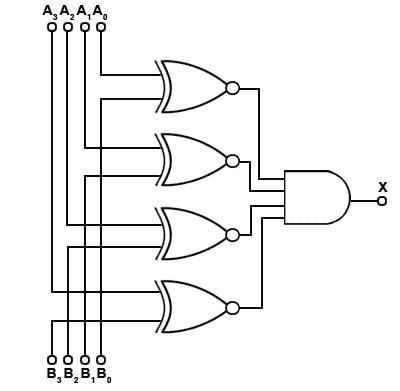
\includegraphics[width=.4\textwidth]{comparador-xnor.jpeg}
\caption{Esquema lógico de um comparador de 4 bits\cite{ref-xnor}}
\label{fig:portas-xnor}
\end{figure}


\subsection{Circuito Debounce}

No ambiente de aprendizagem, para facilitar o entendimento dos circuitos digitais, faz-se uso de artifícios como aproximação e arredondamento. Porém, quando se trata da implementação física, na prática, esses fatos não podem ser ignorados. Como exemplo, um botão ideal, ao ser pressionado, emite um pulso igual ao descrito na figura~\ref{fig:btn-ideal}. Já considerando todas as variáveis presentes no ambiente de prototipagem, testes e uso do produto, o pulso do botão se torna semelhante ao descrito na figura~\ref{fig:btn-real}.

\begin{figure}[!htbp]
\centering
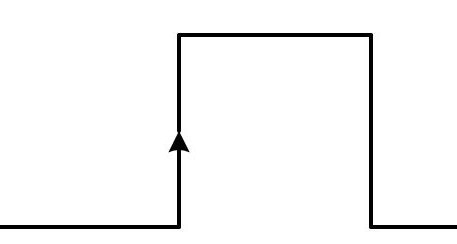
\includegraphics[width=.4\textwidth]{btn-ideal.jpg}
\caption{Pulso de um botão ideal ao ser pressionado\cite{btn-ideal}}
\label{fig:btn-ideal}
\end{figure}


\begin{figure}[!htbp]
\centering
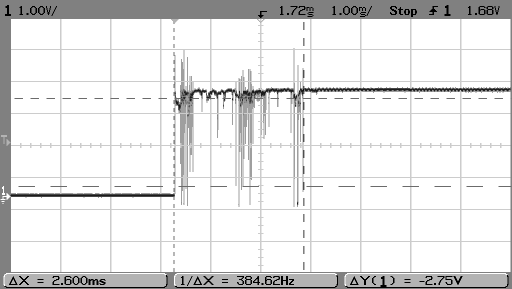
\includegraphics[width=.5\textwidth]{btn-real.png}
\caption{Pulso de um botão real ao ser pressionado\cite{btn-real}}
\label{fig:btn-real}
\end{figure}

Como pode ser visto na figura~\ref{fig:btn-real}, ao ser pressinado, o botão gera uma onda com várias oscilações. O problema dessa variância é que o circuito disparado pelo botão pode ser ativo mais de uma vez quando o mesmo é pressionado apenas uma única vez. A razão disso acontecer é que entre tais oscilações, pode ocorrer uma tão grande que seja capaz de alternar entre os níveis lógicos\cite{debouncing-reason}.

Para garantir que o pulso do botão seja devidamente interpretado, ou seja, que a cada pressionar o disparo apresente uma forma de onda regular, é feito um circuito de \textit{debouncing} que regulariza o pulso proveniente do botão. Tal circuito pode ser feito utilizando multiplicando várias frequências diferentes, sendo que a entrada dos FF's que compõe tal divisor será a saída do botão. Realizando essa operação, a saída será regulada pelas frequências, uma vez ativadas pelo botão, a saída será 1 quando elas todas se encontrarem em pico, atrasando a regularizando o pulso\cite{debouncing-theory}.

Um exemplo do circuito abordado é descrito na figura~\ref{fig:debouncing-ex}, na qual $Sig$ corresponde a entrada do botão, $CLK$ ao clock do sistema e $Deb\_Sig$ ao pulso regularizado pelo circuito.


\begin{figure}[H]
\centering
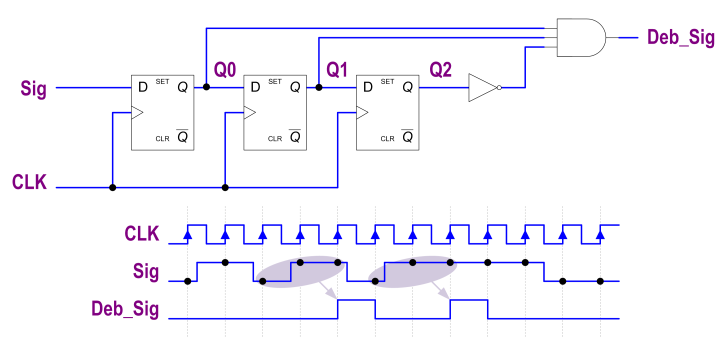
\includegraphics[width=.7\textwidth]{debouncing-ex.png}
\caption{Circuito de Debouncing utilizando FF's D\cite{debouncing-ex}}
\label{fig:debouncing-ex}
\end{figure}

\subsection{Memórias RAM e ROM}

Os computadores e outros tipos de sistemas necessitam de armazenamento permanente ou semi-permanente de uma grande quantidade de dados binários\cite{floyd2011digital}. Para armazenar esses dados, são utilizados dispositivos chamados de memória, sendo os principais tipos as memórias RAM e ROM.

A memória RAM(\textit{Random-Access Memory}), possui capacidade de escrita e gravação e em qualquer ordem, mas os dados são perdidos se a alimentação for desligada, ou seja, são \textit{memórias voláteis}. Esse tipo de memória é composto por módulos básicos de armazenamento, os quais podem ser diretamente acessados por meio de endereçamento\cite{tocci1997digital}. A memória RAM pode ser construída por um conjunto de módulos básicos, sendo que estes são elaborados com FF's. Para que seja funcional, são requeridos, no mínimo, dois dados: o dado de liberação para gravação e o dado a ser gravado. A capacidade de armazenamento da memória RAM, em bits,  vai ser delimitada, no caso básico, pela quantidade de FF's em cada unidade de memória vezes a quantidade de unidades de memória.

A memória ROM(\textit{Read-Only Memory} é um tipo de memória na qual os dados são armazenados permanentemente ou semi-permanentemente. Toda memória ROM possui capacidade de leitura, mas não de escrita e são chamadas de memórias \textit{não voláteis} pelo fato de manter os dados mesmo de a alimentação for desligada. Apesar da nomenclatura, a memória ROM também se trata de uma memória RAM, uma vez que os dados também podem ser acessados de modo aleatório, sendo melhor definida como \textit{memória RAM de apenas leitura}\cite{floyd2011digital}. O tipo mais simples de memória ROM pode ser construído decodificando sinais GCC e GND para obter a saída desejada, e, em seguida, construindo seletores para endereçamento.

\section{Metodologia}
Como definido pela metodologia do PBL, a resolução do problema 3 do MI de Circuitos Digitais, iniciou-se com o levantamento de ideias pelos membros do grupo de quais seriam as possíveis resoluções para o problema. Como de praxe, surgiram diversas ideias sobre como realizar o mesmo procedimento e dúvidas relacionadas ao texto do problema. 

Os membros da sessão, solucionando as questões um dos outros quando possível durante o processo, buscaram tomar decisões de projeto para formalização das obrigações, analisando fatores positivos e negativos das soluções propostas, optando pela solução que fosse mais simples e que estivesse de acordo com o problema, de acordo com a visão dos alunos. Com esse método deu-se início a construção da solução do problema 3 do MI - Circuitos Digitais, começando pela formalização e definição de padrões de projeto e de um diagrama que as mostrasse aplicadas ao circuito.

\subsection{Decisões de Projeto}

Antes de iniciar a implementação do projeto em si, é necessário traçar o caminho a percorrer durante todo o processo de solução do problema. Essa metodologia foi adotada pelos membros da sessão após algumas decisões de projeto que não deram o resultado esperado nos problemas anteriores, causando incongruências entre os módulos projetados entre diferentes membros da turma. 

De início, foi de comum acordo que, mais uma vez, modularizar o problema e dividir tais módulos entre pequenos subgrupos, sendo que cada subgrupo deveria enviar um pequeno relatório contendo todas as informações necessárias para a elaboração do mesmo, para conscientizar os outros alunos do processo de construção, além da descrição do bloco na ferramenta EDA \textit{Quartus II 9.0}. A partir desse ponto, a abordagem mudou em relação aos problemas anteriores, uma vez que houveram problemas com essa segmentação. Para resolver esses problemas de incompatibilidade, a turma resolvou elaborar um diagrama completo do problema, estabelecendo padrões para cada segmento.

\subsection{Elaboração do Diagrama}
Iniciado na primeira sessão do problema 3 e finalizado na segunda sessão do mesmo problema, o diagrama teve como objetivo fazer com que todos os alunos tivessem consciência plena do funcionamento do circuito, da entrada a saída. Descrevendo as relações entre os blocos e a função, a quantidade de entrada e a quantidade de saídas de cada um deles e, também,  padrões de nomenclatura, o diagrama descreve o que cada subgrupo deve fazer para que, quando combinadas, as frações do problema resultem em um circuito funcional e dentro da perspectiva do problema. 

O resultado desse processo de descrição am alto nível do projeto pode ser conferido na figura~\ref{fig:diagrama}, que destaca também as tarefas de cada subgrupo. Por exemplo, o subgrupo amarelo é responsável pela elaboração dos módulos correspondentes ao \textit{decodificador da matriz} e \textit{Bloco do Mux-Coordenada}.

\begin{figure}[H]
\centering
\includegraphics[width=1\textwidth]{diagrama.jpg}
\caption{Diagrama de blocos do Problema 3: Memorizando}
\label{fig:diagrama}
\end{figure}



\subsection{Circuito Debounce}
Circuito utilizado para amenizar a trepidação da onda do botão, recebe como entrada uma frequência de clock dividida resultando em 33$Hz$ e o pulso do botão, e tem como saída um pulso com baixa oscilação caso o botão seja pressionado. A implementação desse circuito pode ser vista na figura~\ref{fig:debounce}.

\begin{figure}[!htbp]
\centering
\includegraphics[width=.7\textwidth]{debounce.png}
\caption{Implementação do circuito Debounce na EDA}
\label{fig:debounce}
\end{figure}


\subsection{Memória ROM}

Necessária para armazenar os dados das coordenadas pré definidas no problema, guarda os dados das coordenadas(linha e coluna) em forma de um arranjo de números binários. Respeitando os endereços fornecidos junto aos pares de coordenadas e convertendo os mesmos para valores binários(demonstrados na tabela~\ref{tab:rom-memory}), foram elaborados os conjuntos de dados a serem programados na memória ROM.

\begin{table}[!htbp]
\centering
\begin{tabular}{||c||c||c||c||}
\hline 
\rule[-1ex]{0pt}{2.5ex} Endereço & Coordenada(CxL) & Valor Binário(C) & Valor Binário(L) \\ 
\hline 
\hline
\rule[-1ex]{0pt}{2.5ex} 0 & B,5 & 1011 & 0101 \\ 
\hline 
\rule[-1ex]{0pt}{2.5ex} 1 & B,1 & 1011 & 0001 \\ 
\hline 
\rule[-1ex]{0pt}{2.5ex} 2 & C,3 & 1100 & 0011 \\ 
\hline 
\rule[-1ex]{0pt}{2.5ex} 3 & D,5 & 1101 & 0101 \\ 
\hline 
\rule[-1ex]{0pt}{2.5ex} 4 & D,1 & 1101 & 0011 \\ 
\hline 
\rule[-1ex]{0pt}{2.5ex} 5 & E,4 & 1110 & 0100 \\ 
\hline 
\rule[-1ex]{0pt}{2.5ex} 6 & E,3 & 1110 & 0011 \\ 
\hline 
\rule[-1ex]{0pt}{2.5ex} 7 & E,2 & 1110 & 0010 \\ 
\hline 
\end{tabular} 
\caption{Informações que devem ser armazenadas e suas versões e binário}
\label{tab:rom-memory}
\end{table}

Para obter os conjuntos de dados desejados, foram dispostos 8 conjuntos de 8 saídas cada, de modo que as saídas de cada conjunto correspondessem aos dados de cada um dos pares de coordenadas. Como pode ser visto na figura~\ref{fig:mem-rom}, as saídas foram nomeadas no padrão $m\alpha b\beta$, onde $\alpha$ corresponde ao endereço de memória e $\beta$ o bit de saída(para $\beta>4$, os bits representam a saída da linha e para $3<\beta<8$ a saída da coluna).

\begin{figure}[!htbp]
\centering
\includegraphics[width=.8\textwidth]{rom-memory.png}
\caption{Descrição da memória ROM na EDA}
\label{fig:mem-rom}
\end{figure}

\subsubsection{Seletor de Memória}
Para efetuar o acesso a memória ROM, é necessário endereçá-la. Buscando isolar os componentes, a turma optou por elaborar um circuito multiplexador que recebe como entrada padrão todas as saídas da memória ROM e, através de 3 seletores $b_{0}, b_{1}, b_{2}$ que devem ser um contador binário de 3 bits, sendo $b_{0}$ o bit menos significativo, põe em uma saída $S$ de 8 bits somente os bits da coordenada de endereço apontado no contador. Para ajudar na tarefa da seleção, sabendo que o contador é um contador binário de 3 bits, foi implementado um decodificador do contador para 8 saídas, cada um representando um endereço e sendo apenas uma ativa por vez. O bloco do multiplexador implementado pode ser visto na ~\ref{fig:mux-mem}.

\begin{figure}[H]
\centering
\includegraphics[width=.9\textwidth]{mem-mux.png}
\caption{Descrição do seletor da memória ROM na EDA}
\label{fig:mux-mem}
\end{figure}

\subsection{Contadores}

Usados para controlar o endereçamento da memória e para oscilar as saídas na Matriz de Leds, os contadores $c_{1}$ e $c_{1}$, respectivamente, são contadores binários síncronos de 3 bits. Por ser responsável pelo endereçamento da memória $c_{1}$ tem como entrada o pulso do botão normalizado pelo Debounce, já $c_{2}$ um pulso de clock dividido de, aproximadamente, 132.8$Hz$. A razão para esse número será explicada em ~\ref{sub:mux-matriz}. 

\subsection{Comparador}
Sendo o tipo de comparador mais simples possível, o comparador utilizado no problema é capaz de comparar dois conjuntos de 8 bits e determinar se eles são iguais ao comparar os bits de mesma magnitude. O comparador presente no problema recebe como entrada o conjunto de dados bruto, oriundo do barramento paralelo de oito bits, e  o conjunto de dados armazenados na unidade da memória ROM correspondente ao endereçamento atual determinado pelo contador $c_{1}$. Ou seja, caso o contador $c_{1}$ esteja em 1, as dados presentes no bloco 1 da memória ROM serão enviados pelo seletor de memória para o comparador.

Como uma característica extra, foi implementado no comparador usado um bit a mais. Tal bit funciona como um $enable$ e é alterado por um botão ligado a um circuito de Debounce.

Sendo $D\_L\alpha$, $D\_L\beta$ e $M\_L\alpha$, $M\_C\beta$ as entradas correspondentes para a entrada do valor inerente linha a coluna disposta no barramento e linha e coluna de referência, respectivamente, o comparados descrito na figura~\ref{fig:comparador} mostra o circuito responsável por comparar coordenadas feito e utilizado pela equipe.

\begin{figure}[H]
\centering
\includegraphics[width=.8\textwidth]{comparador.png}
\caption{Descrição do comparador de coordenadas na EDA}
\label{fig:comparador}
\end{figure}


\subsection{Memória RAM}
A memória RAM, de acordo com o diagrama elaborado, deve receber como bit de ativação o bit de saída do comparador, chamado de $result$ e a saída de $c_{1}$. Caso $result$ esteja em nível alto, esse nível é armazenado no endereço de memória descrito pelo contador $c_{1}$. Caso contrário, nada é feito.

Como uma entrada extra, foi colocada um bit de $clear$ para a memória, o mesmo tem a função de limpar completamente a memória em casos que o $reset$ da mesma seja desejado. A figura~\ref{fig:ram-eda} demonstra o resultado final obtido na ferrmenta EDA, sendo possível perceber o funcionamento, entradas e saídas do respectivo módulo.

\begin{figure}[!htbp]
\centering
\includegraphics[width=.6\textwidth]{ram-eda.png}
\caption{Descrição da memória RAM na EDA}
\label{fig:ram-eda}
\end{figure}

\subsection{Multiplexador da Matriz de LEDs}
Responsável por acender todos os leds, esse item recebe como entrada todos os 8 bits de saída da memória RAM, todas as saídas da memória ROM e as saídas do contador $c_{2}$. A função desse bloco é verificar se, segundo a memória RAM, o endereço $-1<x<8$ foi dado como válido, e caso positivo, acendê-lo, dado que 0 endereço $x$ da memória RAM, informa se o endereço $x$ da ROM foi ativo.

Dado a incapacidade da matriz de LED's de acender 8 LED's simultaneamente, o contador $c_{2}$ alterna entre as 8 coordenadas, liberando o acendimento ou não, de um LED por vez, numa frequência de aproximadamente 132.8$Hz$. Essa frequência foi calculada com base na frequência máxima percebida pelo o olho humano e multiplicando-a por 8, fazendo com que a alternância entre os acendimentos não seja notada a olho-nu.

%IMAGEM

\subsection{Multiplexador do Display Dual de Sete Segmentos} \label{sub:mux-matriz}

No problema anterior, o DSS era responsável apenas por exibir a coordenada na forma de (letra, número) para o usuário. Em discussão, a turma decidiu por implementar um requisito do problema 3 na mesma matriz, sem ferramentas físicas adicionais. As razões para tal escolha foram a economia de material e de tempo refatorando o circuito físico e a aparente facilidade de implementação da solução proposta.

Para exibir o número correspondente ao endereço de memória atual e também as coordenadas, o multiplexador do DSS recebe como entrada todas as saídas do multiplexador do problema 2 e também as saídas do decodificador do contador de $c_{1}$ para decimal. Para realizar a com exatidão, o multiplexador também recebe uma frequência de clock de um período $t=2s$, para tornar a exibição de dois dados em um mesmo display a mais amigável possível.

\subsection{Unificação dos blocos em um projeto}
Com todos os blocos prontos e devidamente testados em ambiente lógico, foram todos unidos em um único projeto e ligados como descrito no diagrama elaborado previamente. Tal tarefa foi destinada a todos os membros da equipe, como a justificativa de fortalecer o conhecimento sobre o problema e comparar e discutir os projetos em caso de eventuais discrepâncias.

\subsection{Refatoração do circuito na protoboard}

Nessa seção é mostrado o resultado da dedicação da equipe aproveitar ao máximo a plataforma física já existente, atribuindo as funções que puder ao circuito lógico. Para efeitos de comparação, constam abaixo a figura~\ref{fig:circuito-p2} e a figura~\ref{fig:circuito-p3}, representando, respectivamente, os circuitos físicos utilizados no problema 2 e no problema 3, respectivamente.

\begin{figure}[!htbp]
\centering
\includegraphics[width=.9\textwidth]{circuito-p2.jpg}
\caption{Circuito físico do problema 2}
\label{fig:circuito-p2}
\end{figure}

\begin{figure}[!htbp]
\centering
\begin{sideways}
\includegraphics[width=.6\textwidth]{circuito-p3.jpg}
\end{sideways}
\caption{Circuito físico do problema 3}
\label{fig:circuito-p3}
\end{figure}

Como é possível ver, a única mudança foi o acréscimo de 3 botões ao sistema. As funções desses botões são, respectivamente, limpar a memória, alterar o endereço de memória e ativar a comparação. Tais alterações foram feitas no Laboratório de Hardware um dia antes do dia marcado para a realização dos teste práticos.

\section{Discussões e resultados}

Nesta sessão serão abordados os principais resultados obtidos, os testes realizados e, além disso, serão abordados alguns detalhes que dizem respeito ao circuito lógico.

\subsection{Testes lógicos no ambiente Quartus II}

Como de praxe, antes realizar os testes físicos, foram realizados testes virtuais com o intuito de avaliar o funcionamento do circuito lógico.  Para realizar esta análise, foram utilizadas ferramentas fornecidas pelo software da Altera, sendo estes os arquivos de WaveForm e o Simulator Tool.

Foram realizados uma série de testes em cada bloco componente do produto final. Todos apresentavam a eficácia pretendida, com a exceção da memória RAM. De início, tal componente não apresentou resultados compatíveis com os desejados e, ao analisar cuidadosamente, foi percebida que a abordagem inicial de usar FF's do tipo D com o D ligado em $VCC$ e utilizar o $result$ do comparador multiplicado com o pulso do botão como clock não daria certo, uma vez que o pulso do botão, mesmo com o Debounce, se mostra irregular. Para corrigir esse erro, o FF foi substituído por um FF do tipo JK com o K aterrado, o J contendo a multiplicação do $result$ com a entrada do botão e a entrada de clock com o clock do sistema. 

Como demonstrado na figura~\ref{fig:teste-ram}, ao receber $result$ em nível alto, estando o $clear$ em estado também alto, a célula de memória passa a armazenar 1 na coordenada apontada pelo contador(o valor em decimal apontado pelo contador corresponde ao endereço da célula de memória). Caso $result$ seja 0, o valor armazenado na célula atual é mantido. Se utilizando da operação de $clear$, toda a memória é limpa e volta ao seu estado primitivo.

\begin{figure}[!htbp]
\centering
\includegraphics[width=1\textwidth]{testeram.png}
\caption{Teste da Memória RAM na EDA}
\label{fig:teste-ram}
\end{figure}

Analisando os requisitos necessários e o comportamento demonstrado pelo dispositivo nos testes, concluiu-se que o mesmo corresponde ao desejado.

\subsection{Funcionamento do Circuito}

O circuito deve receber uma entrada oriunda de um barramento paralelo de oito bits, que deve ser diretamente impressa em um $DSS$, e compará-la com a memória presente no endereço atual, endereço esse que deve também estar sendo impresso em um $DSS$ que alterna as duas informações (coordenadas e endereçamento) para exibição. Caso a entrada e os dados da memória sejam iguais, o LED correspondente a coordenada inserida deverá ser aceso. O controle de endereçamento e de comparação é dado por meio de dois botões distintos. Além disso, a matriz deve voltar ao estado original quando o botão de $clear$ for selecionado.


\subsection{Testes práticos}
Antes de realizar os testes do circuito na Protoboard, fazia-se necessário fazer a demarcação dos pinos adicionais na ferramenta Quartus II e  gravar o circuito lógico do mesmo na FPGA disponível no laboratório. Após a demarcação dos pinos, realizada com experiência adquirida no problema 1, ligou-se o circuito e a gravação foi feita.


Dispondo-se de todas as ferramentas necessárias, o teste foi realizado introduzindo-se todas as coordenadas possíveis e tentando gravá-las na memória. Inicialmente, ao por em prática todo o planejado, foram grandes as falhas. Exibição da coordenada errada, o DSS não alternava entre seus dois estados e a matriz de LED's não acendia mesmo enviando comparações válidas. Como um resultado das práticas de projeto usadas, boa parte da equipe tinha um alto conhecimento em relação a estrutura do circuito, então, em uma revisão de todo o projeto pelo grupo, percebeu-se que tudo não passou de um descuido na hora de interligar os blocos, pois haviam diversos fios desencaixados ou encaixados no lugar errado.

Após a detecção e correção dos erros citados, o circuito funcionou como o imaginado pelo grupo, exibindo, comparando e alternando tudo que deveria na forma que deveria.


\section{Conclusão}

Observando os requisitos que foram solicitados para o desenvolvimento deste sistema digital, é notório que todas as funcionalidades foram cumpridas. Isto se torna mais concreto devido ao sucesso alcançado através dos testes práticos realizados. Em suma, todos os pré-requisitos para a elaboração do projeto das coordenadas foram obtidos com totalidade.

Tendo sido revisado várias vezes e tentando melhorar quando possível, o grupo chegou num resultado simples e funcional, e, além de tudo, totalmente compatível com o problema anterior.

Além do aspecto técnico, houve uma melhora singular no trabalho em equipe a partir do uso das práticas de projeto citadas. Problemas organizacionais, de incompatibilidade e de centralização de conhecimento, outrora frequêntes, foram eliminados ou amenizados.

Apesar do circuito como um todo estar sendo melhorado, outras possíveis melhorias apontadas no problema anterior continuam não realizadas. Tal fato esclarece que tanto com iniciativas do grupo tanto como exigências do próprio problema, atualizações ainda são possíveis, como o uso de um teclado para a inserção das coordenadas e um aviso de erro mais chamativo, como um aviso sonoro(sugestão que persiste do problema anterior) e a automatização da função $comparar$ e da função $clear$, eliminando botões do sistema e o deixando sua interface com o usuário mais simples.

\section{Referências}

Nessa seção constam os trabalhos utilizados como base teórica que foram necessários para chegar a solução descrita nesse relatório.


\bibliographystyle{sbc}
\bibliography{sbc-template}

\end{document}
